\chapter{Badania}

\section{Przeprowadzone badania}

Badania przeprowadzono dla 5 różnych liczb neuronów w warstwie ukrytej: 20, 30, 40, 50, 60.

\section{Porównanie algorytmów}

\begin{figure}[h!]
	\centering
	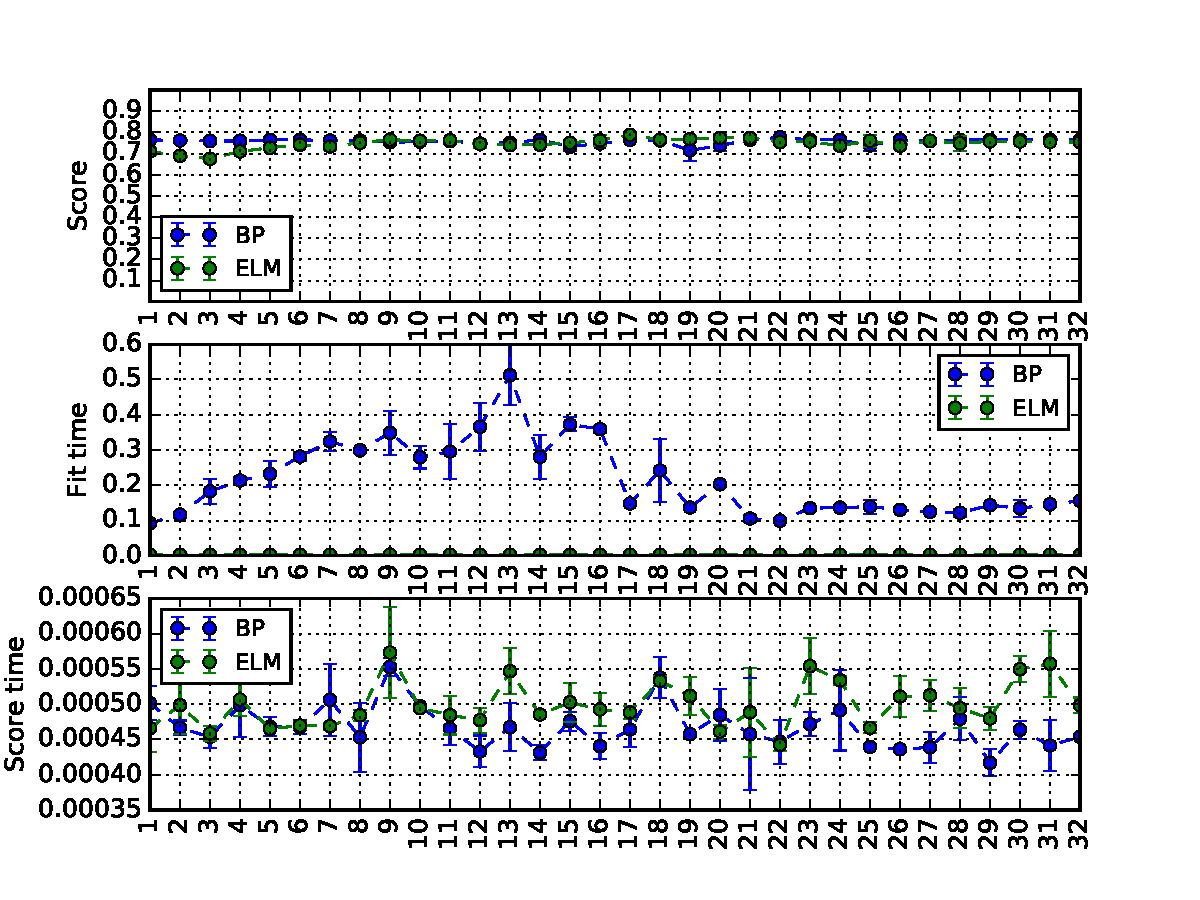
\includegraphics[width=\linewidth]{img/bp_elm_20.pdf}
	\label{Rysunek}
	\caption{20 neuronów w warstwie ukrytej - porównanie obu algorytmów}
\end{figure}

\begin{figure}[h!]
	\centering
	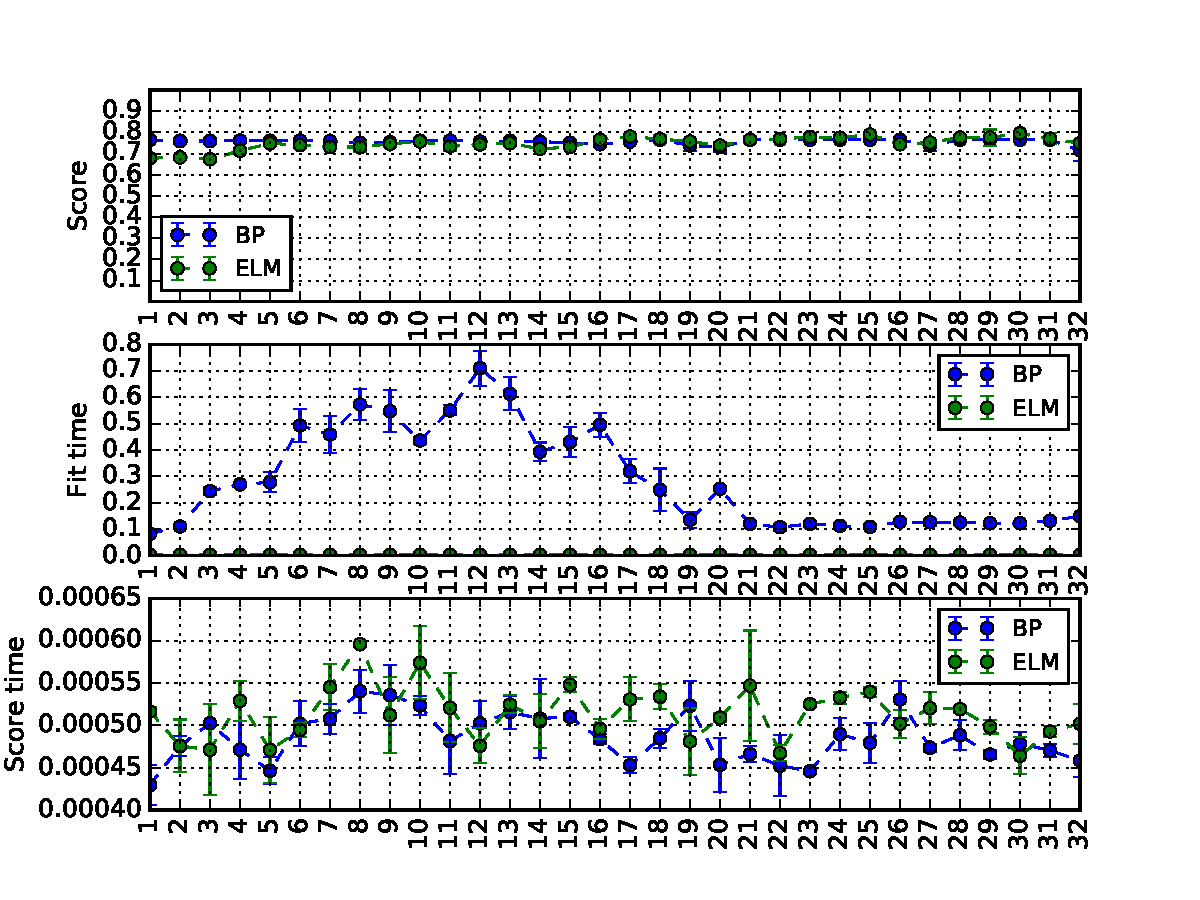
\includegraphics[width=\linewidth]{img/bp_elm_30.pdf}
	\label{Rysunek}
	\caption{30 neuronów w warstwie ukrytej - porównanie obu algorytmów}
\end{figure}

\begin{figure}[h!]
	\centering
	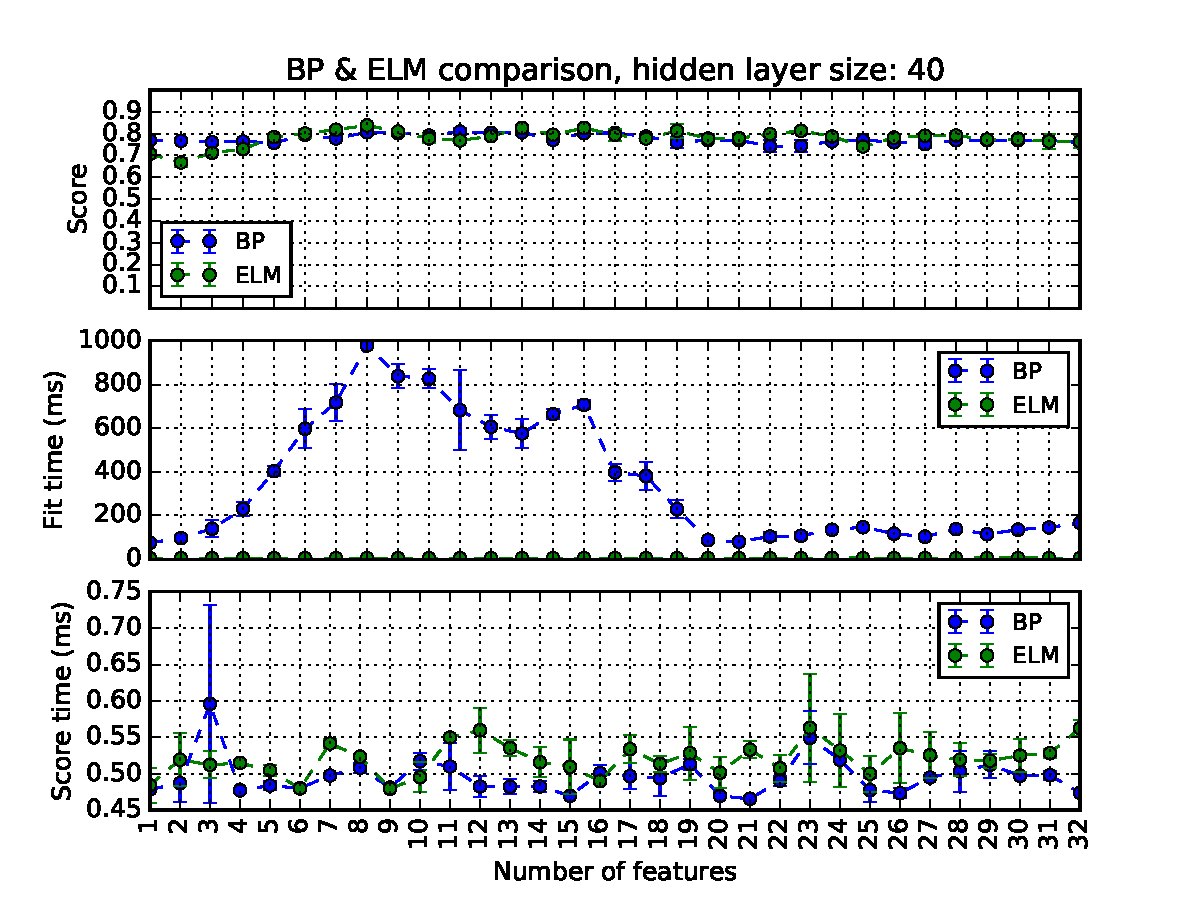
\includegraphics[width=\linewidth]{img/bp_elm_40.pdf}
	\label{Rysunek}
	\caption{40 neuronów w warstwie ukrytej - porównanie obu algorytmów}
\end{figure}

\begin{figure}[h!]
	\centering
	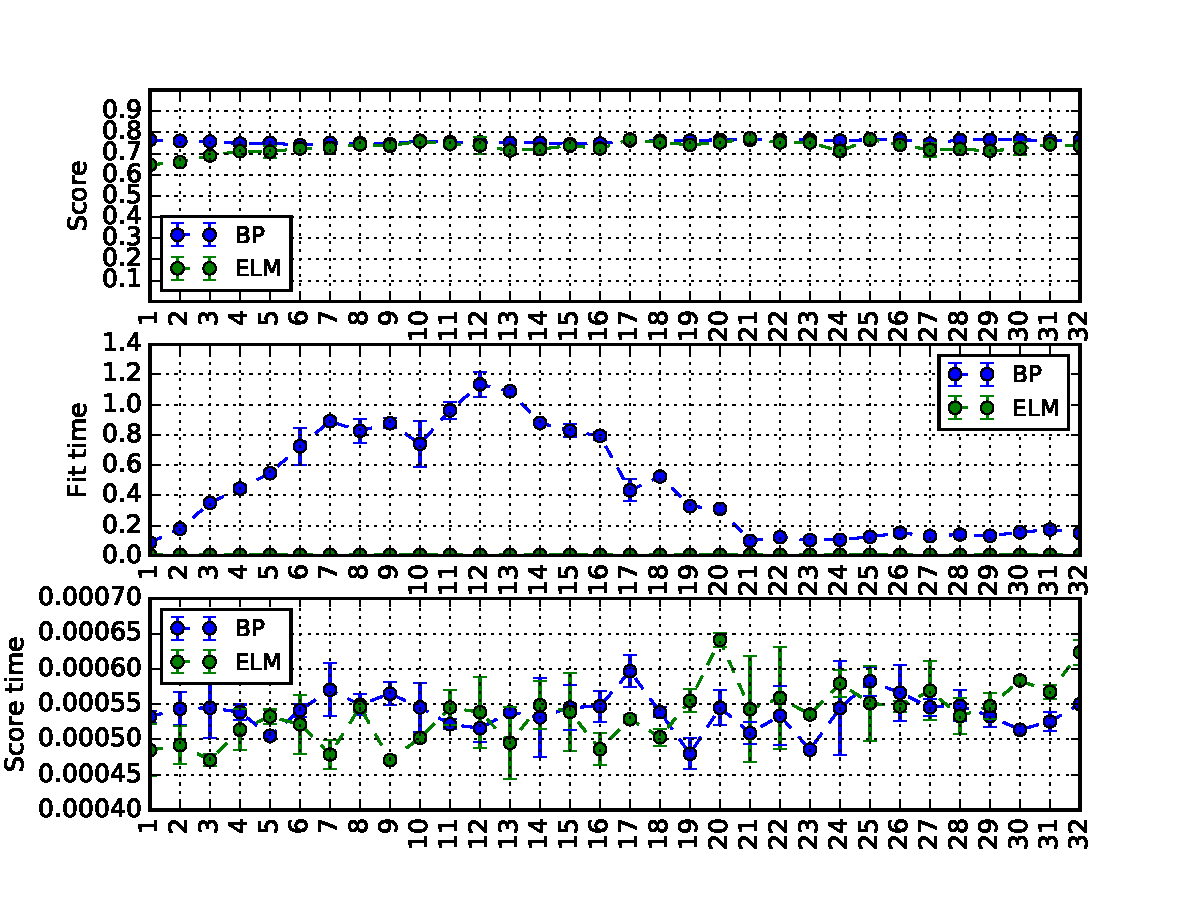
\includegraphics[width=\linewidth]{img/bp_elm_50.pdf}
	\label{Rysunek}
	\caption{50 neuronów w warstwie ukrytej - porównanie obu algorytmów}
\end{figure}

\begin{figure}[h!]
	\centering
	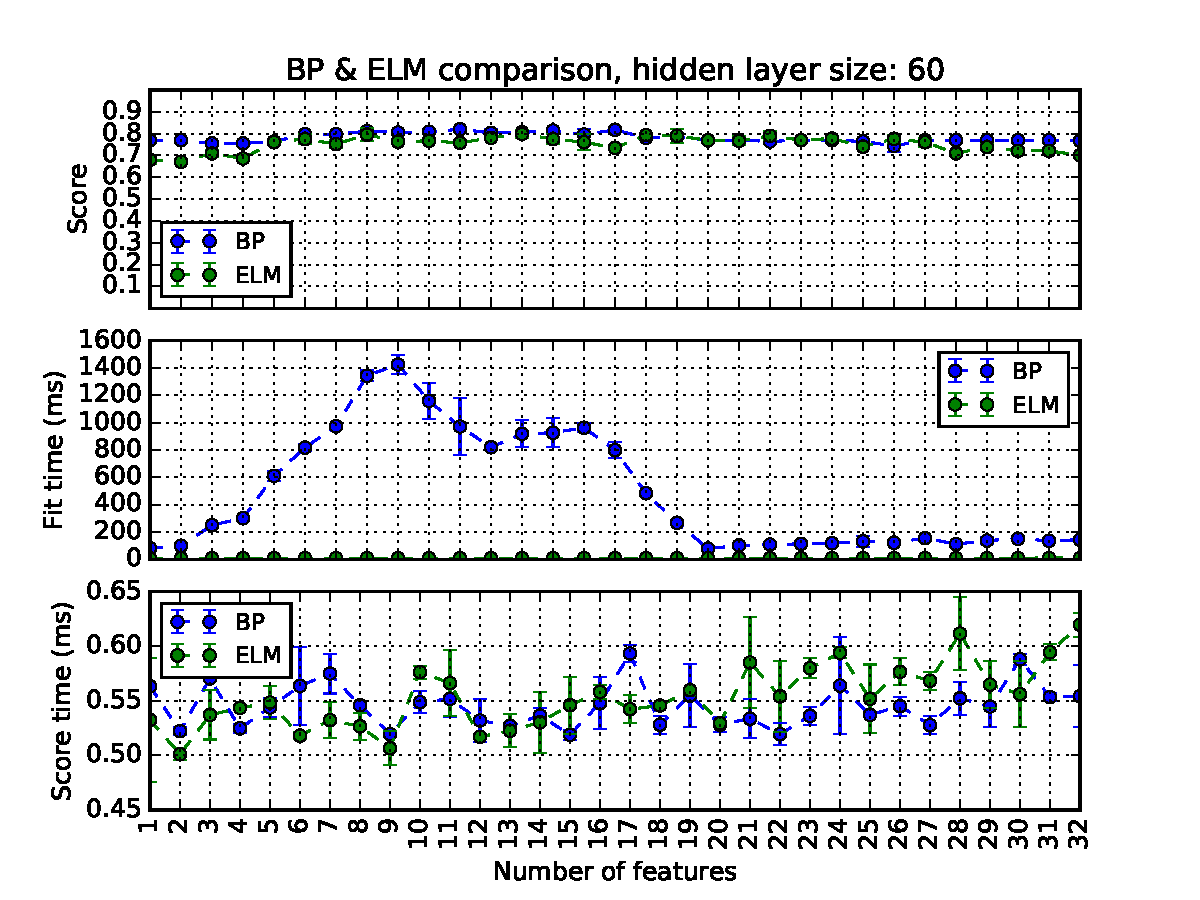
\includegraphics[width=\linewidth]{img/bp_elm_60.pdf}
	\label{Rysunek}
	\caption{60 neuronów w warstwie ukrytej - porównanie obu algorytmów}
\end{figure}

\section{Selekcja cech}
Selekcja cech polega na wybieraniu podzbioru cech w celu ograniczenia czasu uczenia, uproszczenia modelu oraz minimalizacji zjawiska przeuczenia.
\begin{figure}[h!]
	\centering
	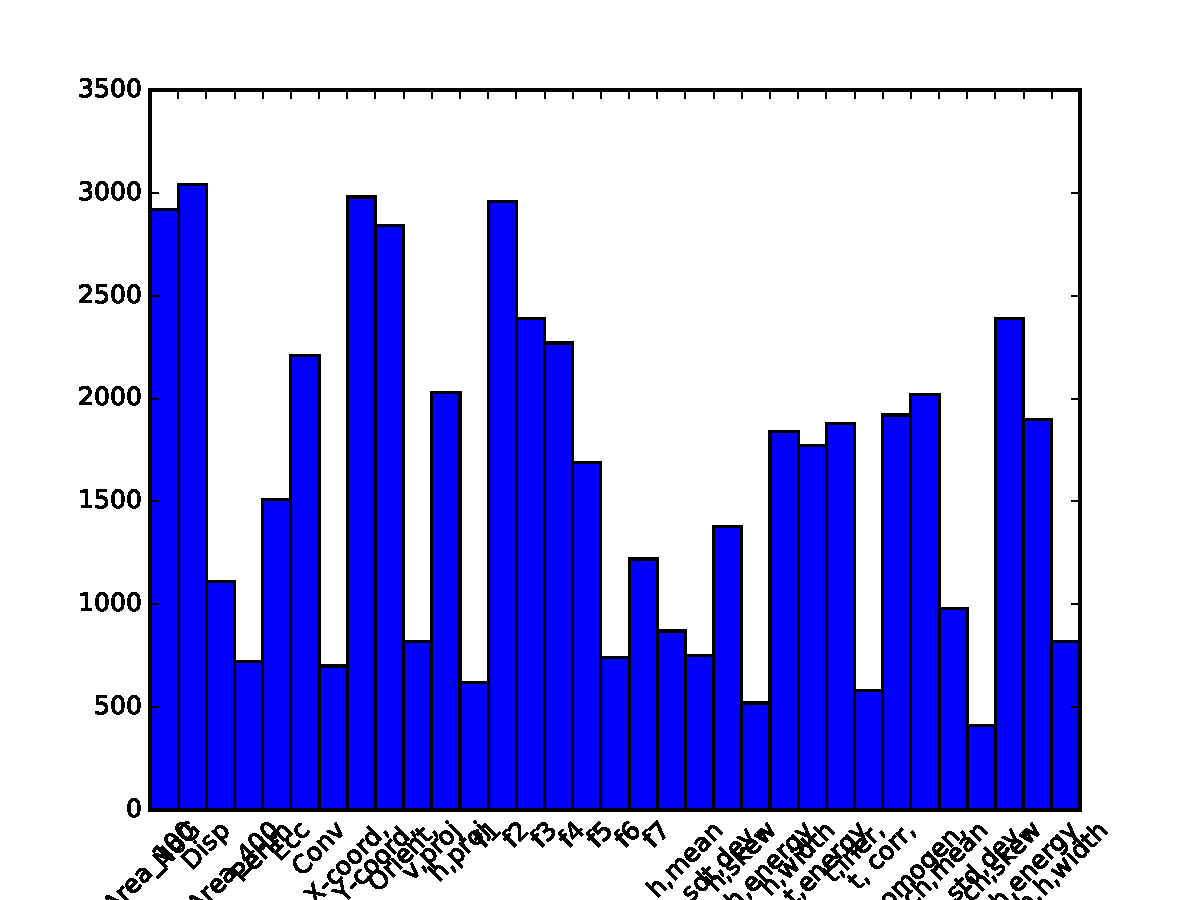
\includegraphics[width=\linewidth]{img/features.pdf}
	\label{Rysunek}
	\caption{Częstość wybierania cech}
\end{figure}

\section{Macierz pomyłek}
Macierz pomyłek umożliwia zobrazowanie jak dobrze klasyfikator radzi sobie ze swoim zadaniem.

Dla problemu z dwiema klasami -- tak jak w aktualnie rozpatrywanym problemie -- macierz dzieli się na cztery części, w których zliczane są obiekty sklasyfikowane poprawnie -- umieszczone na przekątnej macierzy -- oraz błędnie -- umieszczone poza przekątną.
\begin{figure}[h!]
	\centering
	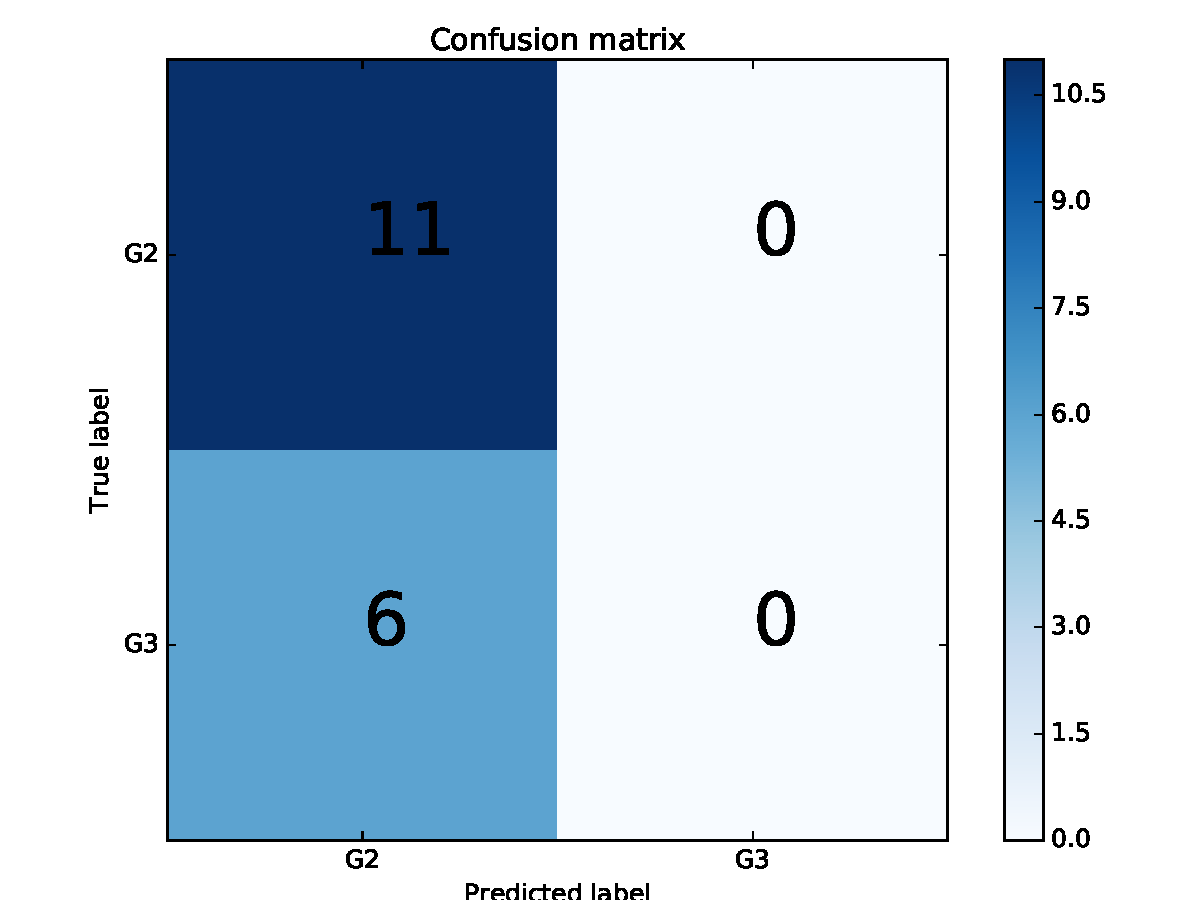
\includegraphics[width=\linewidth]{img/conf_matrix.pdf}
	\label{Rysunek}
	\caption{Przykładowa macierz pomyłek}
\end{figure}